%%%%%%%%%%%%%%%%%%%%%%%%%%%%%%%%%%%%%%%%%%%%%%%%%%%%%%%%%%%%%%%%%%%%%%%%%
% This file is part of the LaTeX sources of the OMDoc 1.3 specification
% Copyright (c) 2016 Michael Kohlhase.
% Source at https://github.com/KWARC/OMDoc/tree/master/doc/spec
% This work is licensed by the Creative Commons Share-Alike license
% see http://creativecommons.org/licenses/by-sa/2.5/ for details
%%%%%%%%%%%%%%%%%%%%%%%%%%%%%%%%%%%%%%%%%%%%%%%%%%%%%%%%%%%%%%%%%%%%%%%%%

\begin{tchapter}[id=complex-theories,short=Complex Theories]{Complex Theories (Module
    \CTHmodule{spec})}

  In \mysecref{theories} we have presented a notion of theory and inheritance that is
  sufficient for simple applications like content dictionaries that informally (though
  presumably rigorously) define the static meaning of symbols. Experience in e.g. program
  verification has shown that this infrastructure is insufficient for large-scale
  developments of formal specifications, where reusability of formal components is the key
  to managing complexity. For instance, for a theory of rings we cannot simply inherit the
  same theory of monoids as both the additive and multiplicative structure.

  In this chapter, we will generalize the \twintoo{inheritance}{relation} from
  \mysecref{theories} to that of ``\indextoo{structure}s'', also called
  ``\twintoo{theory}{morphism}s'' or ``\twintoo{theory}{interpretation}s''
  elsewhere~\cite{Farmer93}.  This infrastructure allows to structure a collection of
  theories into a complex theory graph that particularly supports modularization and reuse
  of parts of specifications and theories. This gives rise to the name ``complex
  theories'' of the \omdoc module.\ednote{All of this chapter is superseded by the MMT
    model, we need to completely rework this! The trick will be to integrate the formal
    (MMT) and informal structures. And we need to get rid of the development graph stuff,
    which MMT can do better.}

\begin{myfig}{cpx-thy}{Complex Theories in \omdoc}
\begin{scriptsize}
  \begin{tabular}{|>{\tt}l|>{\tt}p{1.1truecm}|>{\tt}p{3.3truecm}|c|>{\tt}p{2.9truecm}|}\hline
    {\rm Element}& \multicolumn{2}{l|}{Attributes\hspace*{2.25cm}} & D & Content \\\hline
             & {\rm Required} & {\rm Optional}                  & C &           \\\hline\hline
 theory      &                & xml:id, class, style            & +  & 
             (\llquote{top-level} | imports | structure)*\\\hline
 structure & from & xml:id, class, style & + & morphism?\\\hline
 morphism    &                & xml:id, base, class, style, hiding, type, consistency, exhaustivity & -- & 
                                requation+, measure?, ordering? \\\hline
\end{tabular}
\end{scriptsize}
\end{myfig}
\ednote{get rid of reqequation in favor of simple definitions}

\begin{tsection}[id=morphisms]{Structures: Inheritance via Translations}
  Literal inheritance of symbols is often insufficient to re-use mathematical structures
  and theories efficiently. Consider for instance the situation in the elementary
  \twintoo{algebraic}{hierarchy}: for a theory of rings, we should be able to inherit
  the additive group structure from the theory \snippet{group} of groups and the
  structure of a multiplicative monoid from the theory \snippet{monoid}: A ring is a set
  $R$ together with two operations $+$ and $*$, such that $(R,+)$ is a group with unit $0$
  and inverse operation $-$ and $(R^*,*)$ is a monoid with unit $1$ and base set
  $R^*\deq\setst{r\in R}{r\ne 0}$.  Using the literal inheritance regime introduced so
  far, would lead us into a duplication of efforts as we have to define theories for
  semigroups and monoids for the operations $+$ and $*$ (see \myfigref{rings-simple}).
\begin{myfig}{rings-simple}{A Theory of Rings via Simple Inheritance}
\fbox{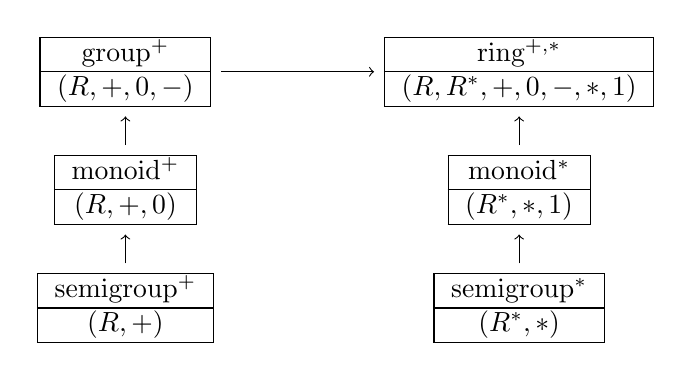
\begin{tikzpicture}
\node (sg) at (1,1)
    {\begin{tabular}{|c|}\hline 
      semigroup$^+$\\\hline
      $(R,+)$\\\hline
    \end{tabular}};
\node (mon) at (1,2.5)
    {\begin{tabular}{|c|}\hline 
      monoid$^+$\\\hline
      $(R,+,0)$\\\hline
    \end{tabular}};
\node (grp) at (1,4)
    {\begin{tabular}{|c|}\hline 
      group$^+$\\\hline
      $(R,+,0,-)$\\\hline
    \end{tabular}};
\node (ring) at (6,4)
    {\begin{tabular}{|c|}\hline 
      ring$^{+,*}$\\\hline
      $(R,R^*,+,0,-,*,1)$\\\hline
    \end{tabular}};
\node (sg1) at (6,1)
    {\begin{tabular}{|c|}\hline 
      semigroup$^*$\\\hline
      $(R^*,*)$\\\hline
    \end{tabular}};
\node (mon1) at (6,2.5)
    {\begin{tabular}{|c|}\hline 
      monoid$^*$\\\hline
      $(R^*,*,1)$\\\hline
    \end{tabular}};

\draw[->](sg)   -- (mon);
\draw[->](sg1)  -- (mon1); 
\draw[->](mon)  -- (grp); 
\draw[->](mon1) -- (ring); 
\draw[->](grp)  -- (ring); 
\end{tikzpicture}}
\end{myfig}
  
This problem\footnote{which seems negligible in this simple example, but in real life,
  each instance of multiple inheritance leads to a \emph{multiplication} of all
  dependent theories, which becomes an exponentially redundant management nightmare.} can
be alleviated by allowing theory inheritance via translations.  Instead of literally
inheriting the symbols and axioms from the source theory, we involve a symbol mapping
function (we call this a \defin{morphism}) in the process. This function maps source
formulae (i.e. built up exclusively from symbols visible in the source theory) into
formulae in the target theory by translating the source symbols.
  
\myfigref{rings-math} shows a theory graph that defines a theory of rings by importing
the monoid axioms via the morphism $\sigma$. With this translation, we do not have to
duplicate the \snippet{monoid} and \snippet{semigroup} theories and can even move the
definition of $\cdot^*$ operator into the theory of monoids, where it intuitively
belongs\footnote{On any monoid $M=(S,\circ,e)$, we have the $\cdot^*$ operator, which
  converts a set $S\subseteq M$ in to $S^*\deq\setst{r\in S}{r\ne e}$}.

\begin{myfig}{rings-math}{A Theory of Rings via Morphisms}
\fbox{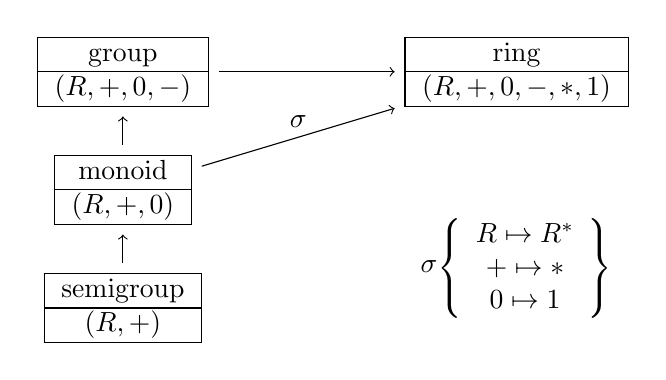
\begin{tikzpicture}
\node (sg) at (1,1)
    {\begin{tabular}{|c|}\hline 
      semigroup\\\hline
      $(R,+)$\\\hline
    \end{tabular}};
\node (mon) at (1,2.5)
    {\begin{tabular}{|c|}\hline 
      monoid\\\hline
      $(R,+,0)$\\\hline
    \end{tabular}};
\node (grp) at (1,4)
    {\begin{tabular}{|c|}\hline 
      group\\\hline
      $(R,+,0,-)$\\\hline
    \end{tabular}};

\node (ring) at (6,4)
    {\begin{tabular}{|c|}\hline 
      ring\\\hline
      $(R,+,0,-,*,1)$\\\hline
    \end{tabular}};
\node (sig) at (6,1.5)
   {$\sigma\deq\scriptscriptstyle\left\{\begin{array}{c}
      R\mapsto R^*\\+\mapsto *\\0\mapsto 1
    \end{array}\right\}$};

\draw[->](sg) -- (mon);
\draw[->](mon) -- (grp);
\draw[->](mon) -- node[above] {$\sigma$} (ring);
\draw[->](grp) -- (ring);
\end{tikzpicture}}
\end{myfig}

Formally, we extend the notion of inheritance given in \mysecref{theories} by
allowing a \twintoo{target}{theory} to import another a \twintoo{source}{theory}
\defin{via a morphism}: Let $\cS$ be a theory with theory-constitutive
elements\footnote{which may in turn be inherited from other theories} $t_1,\ldots,t_n$ and
$\sigma\colon\cS\to\cT$ a morphism, if we declare that $\cT$ imports $\cS$ via $\sigma$,
then $\cT$ {\defin{inherit}s} the theory-constitutive statements $\sigma(t_i)$ from
$\cS$. For instance, the theory of rings inherits the \indextoo{axiom}
$\allcdot{x}{x+0=x}$ from the theory of monoids as
$\sigma(\allcdot{x}{x+0=x})=\allcdot{x}{x*1=x}$.

To specify the formula mapping function, module \CTHmodule{spec} extends the
\element{imports} element by allowing it to have a child element \eldef{morphism},
which specifies a formula mapping by a set of recursive equations using the
\element{requation} element described in \mysecref{definitions}. The optional
attribute \attribute{type}{morphism} allows to specify whether the function is really
recursive (value \attval{recursive}{type}{morphism}) or pattern-defined (value
\attval{pattern}{type}{morphism}). As in the case of the \element{definition} element,
termination of the defined function can be specified using the optional child elements
\element{measure} and \element{ordering}, or the optional attributes
\attribute{uniqueness}{morphism} and \attribute{existence}{morphism}, which point to
uniqueness and existence assertions. Consistency\index{consistency} and
\indextoo{exhaustivity} of the recursive equations are specified by the optional
attributes \attribute{consistency}{morphism} and \attribute{exhaustivity}{morphism}.

\Mylstref{rings} gives the \omdoc representation of the theory graph in
\myfigref{rings-math}, assuming the theories in \mylstref{def-group}.

\begin{lstlisting}[label=lst:rings,
  caption={A Theory of Rings by Inheritance Via Renaming},
  index={derive,method,premise}]
<theory xml:id="ring"> 
  <symbol name="times"/><symbol name="one"/> 
  <structure name="add" from="?group"/>
  <structure name="mult" from="?monoid">
    <morphism> 
      <requation> 
        <OMOBJ><OMS cd="monoid" name="set"/></OMOBJ>
        <OMOBJ>
          <OMA><OMS cd="monoid" name="setstar"/>
            <OMS cd="semigroup" name="set"/>
          </OMA>
        </OMOBJ>
      </requation> 
      <requation> 
        <OMOBJ><OMS cd="monoid" name="op"/></OMOBJ>
        <OMOBJ><OMS cd="ring" name="times"/></OMOBJ>
      </requation> 
      <requation>
        <OMOBJ><OMS cd="monoid" name="neut"/></OMOBJ>
        <OMOBJ><OMS cd="ring" name="one"/></OMOBJ>
      </requation> 
    </morphism> 
  </imports> 
  <axiom xml:id="ring.distribution"> 
    <CMP><xthml:p><OMOBJ><OMS cd="semigroup" name="op"/></OMOBJ> distributes over 
      <OMOBJ><OMS cd="ring" name="times"/></OMOBJ> </xhtml:p>
    </CMP> 
  </axiom>
</theory>
\end{lstlisting}

To conserve space and avoid redundancy, \omdoc morphisms need only specify the values of
symbols that are translated; all other symbols are inherited literally.  Thus the set of
symbols inherited by an \element{imports} element consists of the symbols of the source
theory that are not in the domain of the morphism. In our example, the symbols $R$, $+$,
$0$, $-$, $*$, $1$ are visible in the theory of rings (and any other symbols the theory of
semigroups may have inherited). Note that we do not have a name clash from multiple
inheritance.
  
Finally, it is possible to hide symbols from the source theory by specifying them in the
\attribute{hiding}{morphism} attribute. The intended meaning is that the underlying
signature mapping is defined (total) on all symbols in the source theory except on the
hidden ones. This allows to define symbols that are local to a given theory, which helps
achieve data protection. Unfortunately, there is no simple interpretation of hiding in the
general case in terms of formula translations, see~\cite{CoFI:2004:CASL-RM,MAH-06-a} for
details. The definition of hiding used there is more general. The variant used here arises
as the special case where the hiding morphism, which goes against the import direction, is
an inclusion; then the symbols that are not in the image are the hidden ones.  If we
restrict ourselves to hiding defined symbols, then the situation becomes simpler to
understand: A morphism that hides a (defined) symbol $s$ will translate the
theory-constitutive elements of the source theory by expanding definitions. Thus $s$ will
not be present in the target theory, but all the contributions of the theory-constitutive
elements of the source theory will have been inherited. Say, we want to define the concept
of a sorting function, i.e. a function that --- given a list $L$ as input --- returns a
returns a permutation $L'$ of $L$ that is ordered. In the situation depicted in
\myfigref{rest:actualization}, we would the concept of an ordering function (a function
that returns a permutation of the input list that is ordered) with the help of predicates
\snippet{perm} and \snippet{ordered}. Since these are only of interest in the context
of the definition of the latter, they would typically be hidden in order to refrain from
polluting the name space.

As morphisms often contain common prefixes, the \element{morphism} element has an optional
\attribute{base}{morphism} attribute, which points to a chain of
morphisms\twin{morphism}{base}, whose \indextoo{composition} is taken to be the base of
this morphism. The intended meaning is that the new morphism coincides as a function with
the base morphism, wherever the specified pattern do not match, otherwise their
corresponding values take precedence over those in the \twintoo{base}{morphism}.
Concretely, the \attribute{base}{morphism} contains a whitespace-separated list of
\twintoo{URI}{reference}s to \element{structure} elements. Note that the order of the
references matters: they are ordered in order of the path in the local chain, i.e if we
have \snippet{base="\#\llquote{ref1}\ldots \#\llquote{refn}"} there must be theory
inclusions $\sigma_i$ with \snippet{xml:id="}\llquote{refi}\snippet{"}, such that the
target theory of $\sigma_{i-1}$ is the source theory of $\sigma_i$, and such that the
source theory of $\sigma_1$ and the target theory of $\sigma_n$ are the same as those of
the current view.

Finally, the \CTHmodule{spec} module adds two the optional attributes
\attribute{conservativity}{imports} and \attribute{conservativity-just}{imports} to
the \element{imports} element for stating and justifying \indextoo{conservativity}
(see the discussion below).
\end{tsection}

\begin{tsection}[id=views]{Views}
  
  We have seen that inheritance via morphisms provides a powerful mechanism for
  structuring and re-using theories and contexts. It turns out that the distinguishing
  feature of theory morphisms is that all theory-constitutive elements of the source
  theory are valid in the target theory (possibly after translation). This can be
  generalized to obtain even more structuring relations and thus possibilities for reuse
  among theories. Before we go into the \omdoc infrastructure, we will briefly introduce
  the mathematical model (see e.g.~\cite{Hutter:mocsv00} for details).

  A \defin{view} from a \twindef{source}{theory} $\cS$ to a \twindef{target}{theory} $\cT$
  is a mapping $\sigma$ from $\cS$ objects\footnote{Mathematical objects that can be
    represented using the only symbols of the source theory $\cS$.} to those of $\cT$,
  such that for every theory-constitutive statement $\bS$ of $\cS$, $\sigma(\bS)$ is
  provable in $\cT$ (we say that $\sigma(\bS)$ is a \defin{$\cT$-theorem}\index{theorem}).
   
  In \omdoc, we weaken this logical property to a structural one: We say that a
  theory-constitutive statement $\bS$ in theory $\cS$ is
  \twindef{structurally}{included} in theory $\cT$ via $\sigma$, if there is an
  assertional statement\twin{assertional}{element} $\bT$ in $\cT$, such that the content
  of $\bT$ is $\sigma(\bS)$.  Note that strictly speaking, $\sigma$ is only defined on
  formulae, so that if a statement $\bS$ is only given by a \element{CMP}, $\sigma(\bS)$
  is not defined. In such cases, we assume $\sigma(\bS)$ to contain a \element{CMP}
  element containing suitably translated mathematical vernacular. In this view, a
  \atwindef{structural}{theory}{inclusion} from $\cS$ to $\cT$ is a morphism
  $\sigma\colon\cS\to\cT$, such that every theory-constitutive element is structurally
  included in $\cT$.
  
  Note that an \element{imports} element in a theory $\cT$ with source theory $\cS$ as
  discussed in \mysecref{morphisms} induces a theory inclusion from $\cS$ into
  $\cT$\footnote{Note that in contrast to the inheritance relation induced by the
    \element{imports} elements the relation induced by general theory inclusions may be
    cyclic. A cycle just means that the theories participating in it are semantically
    equivalent.} (the theory-constitutive statements of $\cS$ are accessible in $\cT$
  after translation and are therefore structurally included trivially).  We call this kind
  of theory inclusion \defin{definitional}\atwin{definitional}{theory}{inclusion}, since
  it is a theory inclusion by virtue of the definition of the target theory.  For all
  other theory inclusions (we call them {\atwindef{postulated}{theory}{inclusion}s}), we
  have to establish the theory inclusion property by proving the translations of the
  theory-constitutive statements of the source theory (we call these translated formulae
  \twindef{proof}{obligation}).

  The benefit of a theory inclusion is that all {\indextoo{theorem}s},
  \indextoo{proof}s, and \twintoo{proof}{method}s of the source theory can be used
  (after translation) in the target theory (see \mysecref{induced-assertions}).
  Obviously, the transfer approach only depends on the theorem inclusion property, and we
  can extend its utility by augmenting the theory graph by more theory morphisms than just
  the definitional ones (see~\cite{FaGu93} for a description of the {\imps} theorem
  proving system that makes heavy use of this idea).  We use the infrastructure presented
  in this chapter to structure a collection of theories as a \indextoo{graph} --- the
  \twindef{theory}{graph} --- where the nodes are theories and the links are theory
  inclusions (definitional and postulated ones).

  We call a theory inclusion $\sigma\colon\cS\to\cT$ \defin{conservative}, iff $\bA$ is
  already a $\cS$-theorem for all $\cT$-theorems of the from $\sigma(\bA)$. If the
  morphism $\sigma$ is the identity, then this means the local axioms in $\cT$ only affect
  the local symbols of $\cT$, and do not the part inherited from $\cS$. In particular,
  conservative extensions of consistent theories cannot be inconsistent. For instance, if
  all the local theory-constitutive elements in $\cT$ are symbol declarations with
  definitions, then conservativity is guaranteed by the special form of the
  definitions. We can specify conservativity of a theory inclusion via the
  \attributeshort{conservativity} attribute. The values
  \attvalshort{conservative}{conservativity} and
  \attvalshort{definitional}{conservativity} are used for the two cases discussed
  above. There is a third value: \attvalshort{monomorphism}{conservativity}, which we
  will not explain here, but refer the reader to~\cite{MAH-06-a}.

  \omdoc implements the concept of view in the \indextoo{top-level} \eldef{view}
  element. It has the required attributes \attribute{from}{view} and \attribute{to}{view},
  which point to the source- and target theories and contains a \element{morphism} child
  element as described above to define the translation function. A subsequent (possibly
  empty) set of \element{obligation} elements can be used to mark up proof obligations for
  the theory-constitutive elements of the source theory.

  An \eldef{obligation} is an empty element whose \attribute{assertion}{obligation}
  attribute points to an \element{assertion} element that states that the
  theory-constitutive statement specified by the \attribute{induced-by}{obligation}
  (translated by the morphism in the parent \element{view}) is provable in the target
  theory. Note that a \element{view} element must contain \element{obligation}
  elements for all theory-constitutive elements (inherited or local) of the source theory
  to be correct.

\mylstref{view} shows a theory inclusion from the theory
\snippet{group} defined in \mylstref{def-group} to itself. The morphism just
maps each element of the base set to its inverse. A good application for this kind
of theory morphism is to import claims for symmetric (e.g. with respect to the
function \snippet{inv}, which serves as an involution in \snippet{group})
cases via this theory morphism to avoid explicitly having to prove them (see
\mysecref{induced-assertions}).

\begin{lstlisting}[label=lst:view,mathescape,
  caption={A Theory Inclusion for Groups},
  index={view,morphism,requation,assertion}]
<assertion xml:id="conv.assoc">$\allcdot{x,y,z\in{M}}{z\circ(y\circ x)=(z\circ y)\circ x}$</assertion>
<assertion xml:id="conv.closed" theory="semigroup">$\allcdot{x,y\in{M}}{y\circ x\in{M}}$</assertion>
<assertion xml:id="left.unit" theory="monoid">$\allcdot{x\in{M}}{e\circ x= x}$</assertion>
<assertion xml:id="conv.inv" theory="group">$\allcdot{x,y\in{M}}{x\circ x^{-1}=e}$</assertion>
<view xml:id="grp-conv-grp" from="#group" to="#group">
  <morphism><requation>$X\circ Y\leadsto Y\circ X$</requation></morphism>
  <obligation assertion="#conv.closed" induced-by="#closed.ax"/>
  <obligation assertion="#conv.assoc" induced-by="#assoc.ax"/>
  <obligation assertion="#left.unit" induced-by="#unit.ax"/>
  <obligation assertion="#conv.inv" induced-by="#inv.ax"/>
</view>  
\end{lstlisting}
\end{tsection}

\begin{tsection}[id=restricting-inference,short=Local/Required Theory Inclusions]{Local- and Required Theory Inclusions}
  In some situations, we need to pose well-definedness conditions on theories,
  e.g. that a specification of a program follows a certain security model, or that
  a parameter theory used for actualization satisfies the assumptions made in the
  formal parameter theory; (see \mychapref{natlist} for a discussion). If these
  conditions are not met, the theory intuitively does not make sense. So rather
  than simply stating (or importing) these assumptions as theory-constitutive
  statements --- which would make the theory inconsistent, when they are not met
  --- they can be stated as well-definedness conditions. Usually, these conditions
  can be posited as theory inclusions, so checking these conditions is a purely
  structural matter, and comes into the realm of \omdoc's structural methods.

  \omdoc provides the empty \eldef{inclusion} element for this purpose. It can
  occur anywhere as a child of a \element{theory} element and its
  \attribute{via}{inclusion} attribute points to a theory inclusion, which is
  required to hold in order for the parent theory to be well-defined.
  
  If we consider for instance the situation in
  \myfigref{rest:actualization}\footnote{This example is covered in detail in
    \mychapref{natlist}.}.  There we have a theory \snippet{OrdList} of lists that is
  generic in the elements (which is assumed to be a totally ordered set, since we want to
  talk about ordered lists). We want to to instantiate \snippet{OrdList} by applying it
  to the theory \snippet{NatOrd} of natural numbers and obtain a theory
  \snippet{NatOrdList} of lists of natural numbers by importing the theory
  \snippet{OrdList} in \snippet{NatOrdList}. This only makes sense, if
  \snippet{NatOrd} is a totally ordered set, so we add an \element{inclusion} element
  in the statement of theory \snippet{NatOrdList} that points to a theory inclusion of
  \snippet{TOSet} into \snippet{OrdNat}, which forces us to verify the axioms of
  \snippet{TOSet} in \snippet{OrdNat}.

\begin{myfig}{rest:actualization}{A Structured Specification of Lists (of
    Natural Numbers)}
  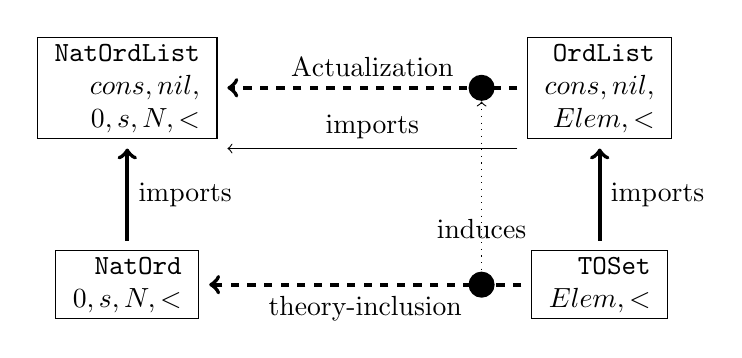
\begin{tikzpicture}  \node (natordlist) at (0,2.5) 
    {\begin{tabular}{|r|}\hline 
      {\tt{NatOrdList}}\\
      $cons, nil,$\\
      $0,s,{\mathbb{N}},<$\\\hline
    \end{tabular}};
  \node (natord) at (0,0) 
    {\begin{tabular}{|r|}\hline 
      {\tt{NatOrd}}\\
      $0,s,{\mathbb{N}},<$\\\hline
    \end{tabular}};
  \node (toset) at (6,0) 
    {\begin{tabular}{|r|}\hline 
      {\tt{TOSet}}\\
      $Elem,<$\\\hline
    \end{tabular}};
  \node (ordlist) at (6,2.5) 
    {\begin{tabular}{|r|}\hline 
      {\tt{OrdList}}\\
      $cons, nil,$\\
      $Elem,<$\\\hline
    \end{tabular}};
  \node[circle,fill] (act1) at (4.5,2.5) {};
  \node[circle,fill] (act2) at (4.5,0) {};
  \draw [->,line width=1.5pt] (natord) -- node[right]{imports} (natordlist);
  \draw [->,line width=1.5pt] (toset) -- node[right]{imports} (ordlist);
  \draw [->,dashed,line width=1.5pt] (toset) -- node[below]{theory-inclusion} (natord);
  \draw [->,dashed,line width=1.5pt] (ordlist) -- node[above]{Actualization} (natordlist);
  \draw [->] (ordlist.south west) -- node[above]{imports} (natordlist.south east);
  \draw [<-,dotted,near end] (act1) -- node{induces} (act2);
\end{tikzpicture}\quad
  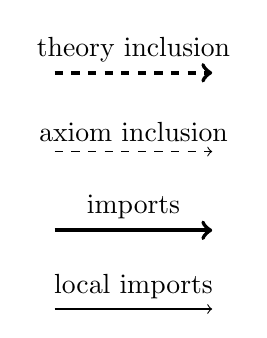
\begin{tikzpicture}
    \draw[->,dashed,line width=1.5pt] (0,3) -- node[above]{theory inclusion} (2,3);
    \draw[->,dashed] (0,2) -- node[above]{axiom inclusion} (2,2);
    \draw[->,line width=1.5pt] (0,1) -- node[above]{imports} (2,1);
    \draw[->] (0,0) -- node[above]{local imports} (2,0);
 \end{tikzpicture}
\end{myfig}

Furthermore note, that the inclusion of \snippet{OrdList} into \snippet{NatOrdList}
should not include the \snippet{TOSet} axioms on orderings, since this would defeat the
purpose of making them a precondition to well-definedness of the theory
\snippet{NatOrdList}. Therefore \omdoc follows the ``development graph model'' put
forward in~\cite{Hutter:mocsv00} and generalizes the notion of theory inclusions even
further: A formula mapping between theories $\cS$ and $\cT$ is called a
\atwindef{local}{theory}{inclusion} or \twindef{axiom}{inclusion}, if the theory
inclusion property holds for the local theory-constitutive statements of the source
theory.  To distinguish this from the notion of a proper \twintoo{theory}{inclusion} ---
where the theory inclusion property holds for all theory constitutive statements of $\cS$
(even the inherited ones) --- we call the latter one \defin{global}. Of course all
global theory inclusions are also local ones, so that the new notion is a true
generalization. Note that the structural inclusions of an \twintoo{axiom}{inclusion} are
not enough to justify translated source theorems in the target theory.

To allow for a local variant of inheritance, the \CTHmodule{spec} module adds an
attribute \attribute{type}{imports} to the \element{imports} element. This can take
the values \attval{global}{type}{imports} (the default) and
\attval{local}{type}{imports}. In the latter case, only the theory-constitutive
statements that are local to the source theory are imported.
  
Furthermore, the \CTHmodule{spec} module introduces the \eldef{axiom-inclusion}
element for \atwintoo{local}{theory}{inclusion}s. This has the same attributes as
\element{view}: \attribute{from}{axiom-inclusion} to specify source
theory, \attribute{to}{axiom-inclusion} for the target theory. It also allows
\element{obligation} elements as children.
\end{tsection}

\begin{tsection}[id=induced-assertions,short=Induced Assertions]{Induced Assertions and Expositions}
  The main motivation of theory inclusions is to be able to transport mathematical
  statements from the \twintoo{source}{theory} to the \twintoo{target}{theory}. In
  \omdoc, this operation can be made explicit by the attributes
  \attributeshort{generated-from} and \attributeshort{generated-via} that the module
  \CTHmodule{spec} adds to all \twintoo{mathematical}{statement}s.  On a statement
  $\bT$, the second attribute points to a \twintoo{theory}{inclusion} $\sigma$ whose
  target is (imported into the) current theory, the first attribute points to a statement
  $\bS$ in that theory which is of the same type (i.e. has the same \omdoc element name)
  as $\bT$.  The content of $\bT$ must be (equivalent to) the content of $\bS$ translated
  by the morphism of $\sigma$.
  
  In the context of the theory inclusion in \mylstref{view}, we
  might have the following situation:
\begin{lstlisting}[label=lst:assertion-translation,mathescape,
  caption={Translating a Statement via a Theory Inclusion},
  index={translated-from,translated-via}]
<assertion xml:id="foo" type="theorem">$\ldots$</assertion>
<proof xml:id="foo.pf" for="#foo">$\ldots$</proof>
<assertion xml:id="target" induced-by="#foo" induced-via="#grp-conv-grp"> 
  $\ldots$
</assertion>
\end{lstlisting}
Here, the second assertion is induced by the first one via the theory inclusion in
\mylstref{view}, the statement of the theorem is about the inverses.  In
particular, the proof of the second theorem comes for free, since it can also be induced
from the proof of the first one.

In particular we see that in \omdoc documents, not all statements are automatically
generated by translation e.g. the proof of the second assertion is not explicitly stated.
Mathematical knowledge management systems like knowledge bases might choose to do so, but
at the document level we do not mandate this, as it would lead to an explosion of the
document sizes. Of course we could cache the transformed proof giving it the same ``cache
attribute state''.

Note that not only statements like assertions and proofs can be translated via theory
inclusions, but also whole documents: Say that we have course materials for elementary
algebra introducing monoids and groups via \twintoo{left}{unit}s and
\twintoo{left}{inverse}s, but want to use examples and exercises from a book that
introduces them using \twintoo{right}{unit}s and \twintoo{right}{inverse}s. Assuming
that both are formalized in \omdoc, we can just establish a theory morphism much like
the one in \mylstref{view}. Then we can automatically translate the
exercises and examples via this theory inclusion to our own setting by just applying the
morphism to all formulae in the text\footnote{There may be problems, if mathematical
  statements are verbalized; this can currently not be translated directly, since it would
  involve language processing tools much beyond the content processing tools described in
  this {\report}. For the moment, we assume that the materials are written in a controlled
  subset of mathematical vernacular that avoids these problems.}  and obtain exercises and
examples that mesh well with our introduction. Of course there is also a theory inclusion
in the other direction, which is an inverse, so our colleague can reuse our course
materials in his right-leaning setting.

Another example is the presence of different normalization factors in physics or branch
cuts in elementary complex functions. In both cases there is a plethora of definitions,
which all describe essentially the same objects (see e.g.~\cite{BraCor:raefca02} for an
overview over the branch cut situation). Reading materials that are based on the ``wrong''
definition is a nuisance at best, and can lead to serious errors. Being able to adapt
documents by translating them from the author theory to the user theory by a previously
established theory morphism can alleviate both.

Mathematics and science are full of such situations, where objects can be viewed from
different angles or in different representations. Moreover, no single representation is
``better'' than the other, since different views reveal or highlight different aspects of
the object (see~\cite{KohKoh:esmk05} for a systematic account). Theory inclusions seem
uniquely suited to formalize the structure of different views in mathematics and their
interplay, and the structural markup for theories in \omdoc seems an ideal platform for
offering added-value services that feed on these structures without committing to a
particular formalization or foundation of mathematics.
\end{tsection}

\end{tchapter}
%%% Local Variables: 
%%% mode: latex
%%% TeX-master: "omdoc"
%%% End: 

% LocalWords:  cpx def requation lst setstar cd mathescape ti thi cic bic aic
% LocalWords:  aia im axa xunit linewidth arcangle ai ima imb axb axc param ord
% LocalWords:  elem toset nat elt nats incl morph natlist dec adt  sg dg truecm
% LocalWords:  mon grp mult tn  TOSet NatOrd sortdef TOset CMP FMP pspic TOSet
% LocalWords:  pt linestyle omdoc elal dgraph conv xref yunit ref ic tcic ns th
% LocalWords:  cpx def requation lst setstar cd mathescape ti thi cic bic aic
% LocalWords:  aia im axa xunit linewidth arcangle ai ima imb axb axc param ord
% LocalWords:  elem toset nat elt nats incl morph natlist dec adt  sg ref conv
% LocalWords:  mon grp mult tn  TOSet NatOrd sortdef TOset OrdList OrdNat TOSet
% LocalWords:  NatOrdList pf attr sig OMOBJ OMA globals refi inv TOSet TOSet
% LocalWords:  TOSet TOSet TOSet TOSet TOSet TOSet TOSet TOSet TOSet TOSet foo
% LocalWords:  Hutter mocsv00 conv.assoc assoc.ax BraCor raefca02 KohKoh esmk05
